%%
%% This is file `sample-sigplan.tex',
%% generated with the docstrip utility.
%%
%% The original source files were:
%%
%% samples.dtx  (with options: `sigplan')
%% 
%% IMPORTANT NOTICE:
%% 
%% For the copyright see the source file.
%% 
%% Any modified versions of this file must be renamed
%% with new filenames distinct from sample-sigplan.tex.
%% 
%% For distribution of the original source see the terms
%% for copying and modification in the file samples.dtx.
%% 
%% This generated file may be distributed as long as the
%% original source files, as listed above, are part of the
%% same distribution. (The sources need not necessarily be
%% in the same archive or directory.)
%%
%%
%% Commands for TeXCount
%TC:macro \cite [option:text,text]
%TC:macro \citep [option:text,text]
%TC:macro \citet [option:text,text]
%TC:envir table 0 1
%TC:envir table* 0 1
%TC:envir tabular [ignore] word
%TC:envir displaymath 0 word
%TC:envir math 0 word
%TC:envir comment 0 0
%%
%%
%% The first command in your LaTeX source must be the \documentclass command.
\documentclass[sigplan, 10pt, anonymous, review]{acmart}\settopmatter{printfolios=true,printccs=false,printacmref=false}

%%
%% \BibTeX command to typeset BibTeX logo in the docs
\AtBeginDocument{%
  \providecommand\BibTeX{{%
    \normalfont B\kern-0.5em{\scshape i\kern-0.25em b}\kern-0.8em\TeX}}}

%% Rights management information.  This information is sent to you
%% when you complete the rights form.  These commands have SAMPLE
%% values in them; it is your responsibility as an author to replace
%% the commands and values with those provided to you when you
%% complete the rights form.
\setcopyright{acmcopyright}
\copyrightyear{2018}
\acmYear{2018}
\acmDOI{10.1145/1122445.1122456}

%% These commands are for a PROCEEDINGS abstract or paper.
\acmConference[Woodstock '18]{Woodstock '18: ACM Symposium on Neural
  Gaze Detection}{June 03--05, 2018}{Woodstock, NY}
\acmBooktitle{Woodstock '18: ACM Symposium on Neural Gaze Detection,
  June 03--05, 2018, Woodstock, NY}
\acmPrice{15.00}
\acmISBN{978-1-4503-XXXX-X/18/06}


%%
%% Submission ID.
%% Use this when submitting an article to a sponsored event. You'll
%% receive a unique submission ID from the organizers
%% of the event, and this ID should be used as the parameter to this command.
%%\acmSubmissionID{123-A56-BU3}

%%
%% The majority of ACM publications use numbered citations and
%% references.  The command \citestyle{authoryear} switches to the
%% "author year" style.
%%
%% If you are preparing content for an event
%% sponsored by ACM SIGGRAPH, you must use the "author year" style of
%% citations and references.
%% Uncommenting
%% the next command will enable that style.
%%\citestyle{acmauthoryear}

%%
%% end of the preamble, start of the body of the document source.
\begin{document}

%%
%% The "title" command has an optional parameter,
%% allowing the author to define a "short title" to be used in page headers.
\title{Verification of OpenSSL's SHA3 Keccak function using the Software Analysis Workbench}

%%
%% The "author" command and its associated commands are used to define
%% the authors and their affiliations.
%% Of note is the shared affiliation of the first two authors, and the
%% "authornote" and "authornotemark" commands
%% used to denote shared contribution to the research.
\author{Benjamin Winters}
\author{Parker Hanson}
\author{Eric Mercer}
\email{egm@cs.byu.edu}
\orcid{0000-0002-2264-2958}
\author{Brett Decker}
\email{bdecker@cs.byu.edu}
\affiliation{%
  \institution{Brigham Young University}
  \streetaddress{3365 TMCB}
  \city{Provo}
  \state{Utah}
  \country{USA}
  \postcode{84602}
}

%%
%% By default, the full list of authors will be used in the page
%% headers. Often, this list is too long, and will overlap
%% other information printed in the page headers. This command allows
%% the author to define a more concise list
%% of authors' names for this purpose.

%%
%% The abstract is a short summary of the work to be presented in the
%% article.

\shaThree\ is the new standard from \nist\ for computing digests. 
\openssl\ is one of the most widely used implementations of cryptographic protocols.
\cryptol\ and the Software Analysis Workbench (\saw) are a language and verification engine to specify cryptographic primitives and prove equivalence to implementations.
As digests are the basis for all cryptographic protocols, the research in this paper is an automated \saw\ proof of equivalence between the \shaThree\ standard and the actual \openssl\ implementation in C.
The research contributes \cryptol\ specifications for the published standard and the \openssl\ implementation of the standard with its several changes.
The equivalence proof shows the importance of overrides in \saw\ to replace C code with \cryptol\ to reduce the complexity of the proof obligations that must be accomplished relative to the implementation in C.
The research establishes the viability of verifying modern cryptographic primitives and the importance of modularity in their definitions, and implementations, for overrides.

% The \keccak\ function in the SHA-3 NIST standard is responsible for the major computations of all SHA-3 hash constructs.
% These constructs form the basis for modern secure hashing.
% This work extends and improves the methodology used to verify Amazon's s2n HMAC and OpenSSL's SHA2-256 inner hash function. 
% It uses the Software Analysis Workbench (SAW) to prove out functional equivalence between OpenSSL's SHA-3 Keccak function and a verified implementation of SHA-3 in Cryptol, a domain-specific language for cryptography. 
% SAW allows for a modular approach to writing proofs through the use of contracts, which define a functions input to output relationship.
% Each contract, also called an override, is an obligation in the full proof.
% This work leverages SAW by creating overrides to decompose computation and create a compositional proof that is within the capacity of an SMT solver. 
% Visual inspection between Cryptol and the NIST standard is simplified through the creation of Cryptol utility functions.
% These utility functions wrap the complex list comprehensions required for looping in Cryptol.
% The results of this work indicates that a modular approach in cryptographic algorithm design greatly simplifies the verification process, as exemplified by SHA-3.




%%NEED TO COMPLETE THIS BEFORE SUBMISSION
%% The code below is generated by the tool at http://dl.acm.org/ccs.cfm.
%% Please copy and paste the code instead of the example below.
%%
\begin{CCSXML}
<ccs2012>
 <concept>
  <concept_id>10010520.10010553.10010562</concept_id>
  <concept_desc>Computer systems organization~Embedded systems</concept_desc>
  <concept_significance>500</concept_significance>
 </concept>
 <concept>
  <concept_id>10010520.10010575.10010755</concept_id>
  <concept_desc>Computer systems organization~Redundancy</concept_desc>
  <concept_significance>300</concept_significance>
 </concept>
 <concept>
  <concept_id>10010520.10010553.10010554</concept_id>
  <concept_desc>Computer systems organization~Robotics</concept_desc>
  <concept_significance>100</concept_significance>
 </concept>
 <concept>
  <concept_id>10003033.10003083.10003095</concept_id>
  <concept_desc>Networks~Network reliability</concept_desc>
  <concept_significance>100</concept_significance>
 </concept>
</ccs2012>
\end{CCSXML}

\ccsdesc[500]{Computer systems organization~Embedded systems}
\ccsdesc[300]{Computer systems organization~Redundancy}
\ccsdesc{Computer systems organization~Robotics}
\ccsdesc[100]{Networks~Network reliability}

%%
%% Keywords. The author(s) should pick words that accurately describe
%% the work being presented. Separate the keywords with commas.
\keywords{verification, cryptography, symbolic execution, SHA3}

%% A "teaser" image appears between the author and affiliation
%% information and the body of the document, and typically spans the
%% page.
% \begin{teaserfigure}
%   \includegraphics[width=\textwidth]{sampleteaser}
%   \caption{Seattle Mariners at Spring Training, 2010.}
%   \Description{Enjoying the baseball game from the third-base
%   seats. Ichiro Suzuki preparing to bat.}
%   \label{fig:teaser}
% \end{teaserfigure}

%%
%% This command processes the author and affiliation and title
%% information and builds the first part of the formatted document.
\maketitle

This paper discusses an automated proof of the \emph{Secure Hash Algorithm 3} (\shaThree) in \openssl\ using the \emph{Software Analysis Workbench} (\saw) by Galois.
\shaThree\ is the latest algorithm for computing \emph{digests}, or hashes, from data to be published by the \emph{National Institute of Standards and Technology} (\nist).
The algorithm is the successor to \shaTwo.
Its intent is to address weaknesses in \shaTwo, and it departs from its predecessors in that it is based on the \keccak\ family of cryptographic primitives \cite{fips202}.

\openssl\ is a commercial grade free cryptographic library \cite{openssl}.
Its implementation of the \emph{Secure Sockets Layer} (SSL) and \emph{Transport Layer Security} protocols are widely deployed on internet facing applications.
Computing digests is a critical operation in these protocols and is the basis to the security guarantees provided by these protocols.
Widely deployed implementations, such as \openssl, are especially important to be correct because of the available attack surface to hackers if a vulnerability were discovered in such implementations.
The seriousness of getting these implementations correct is recently seen in the Apache \texttt{log4j} vulnerability affecting virtually all internet facing servers \cite{log4j}.

\saw\ is a formal verification tool to prove equivalence between \sawcore\ models. \sawcore\ models are defined in the \cryptol\ functional language or extracted from C or Java with \emph{symbolic execution}.
\cryptol\ itself is designed to specify cryptographic primitives at the bit level.
\saw\ has been shown capable in proving implementations of cryptographic primitives equivalent to hardware and software implementations \cite{crypt-hi,hard-soft,design-verif}.
Recent work emphasizes not just the utility of \saw, but the importance of modular decomposition of cryptographic primitives in their definition as that decomposition lends itself to efficient verification in \saw\ \cite{nfm-us}. 

This paper details another example of \saw\ verification only this time it is a proof showing the \openssl\ C implementation of \shaThree\ matches a \cryptol\ specification derived from the published \fips\ standard by \nist\ \cite{fips202}.
The \cryptol\ specifications, \saw\ scripts, and extracted \sawcore\ model from the \openssl\ C implementation are documented, and available, in a public GitHub repository for independent verification \cite{sha3proof}.
The proof relies on two specifications, both created as part of this research, of the \shaThree\ algorithm: one that closely matches the published standard and another incorporating features in the C implementation.
\saw\ shows an input to output equivalence between these two specifications for the 256 bit digest over a fixed set of message sizes. The proof takes around 60 hours of computation time.

The proof then turns to the inner \keccak\ function that computes the actual bits for the digest.
Here it shows that the C implementation exactly matches the \cryptol\ specification on any input.
The proof requires the use of \emph{overrides} in \saw\ to simplify the extracted model from C after symbolic execution.
The proof of equivalence between the \keccak\ in C and \cryptol\ takes around 15 minutes of computation time.

The proof, with its artifacts in the published repository, make the following contributions:
\begin{compactitem}
  \item \cryptol\ for \shaThree\ that passes the test vectors and correlates with \fips.
  \item \cryptol\ for \shaThree\ that uses a reordered memory layout and precomputed tables that correlate with C implementations.
  \item A \saw\ proof showing the two specifications equivalent for the 256 bit digest over a series of message sizes.
  \item A \saw\ proof that the \keccak\ specification in \cryptol\ is equivalent to the \openssl\ C implementation of the same function for all inputs.
\end{compactitem}
The proof shows that \saw\ is capable of proving equivalence to C implementations of modern cryptographic primitives.
It also shows that the modular definition of \shaThree\ naturally lends itself to formal verification in \saw.
The work in its entirety argues the importance of using formal languages such as \cryptol\ for the specification of cryptographic primitives rather than English prose and math.
It also argues the necessity, and viability, of proving at the intermediate representation level equivalence between cryptographic specifications and actual C implementations.

\begin{comment}
\noindent \textbf{Limitations}
\begin{compactitem}
  \item Visual inspection and limited test vectors for (1) and (2)
  \item Only provide proof certificates for message sizes of X to Y for digest sizes of \textbf{FIXME} for (3)
  \item Visual inspection only for anything above Keccak for (3) in OpenSSL's C-code
\end{compactitem}

\subsection{Related Work}
  Previously, Galois' Inc. worked with Amazon to prove out parts of Amazon's s2n HMAC code to the NIST specification.  
In their work they stubbed out use of the SHA2 algorithm because their HMAC allows for customization of the algorithm type and implementation.

The work by Decker et. al, extended on Galois' work by choosing a single SHA2 implementation to prove out.  
They chose OpenSSL's SHA 256 implementation, as that is a commonly used library (and one that is usable in s2n).  
They were able to prove out the inner hash computations of that implementation using a methodology of compositional proofs to do so.  
They were also able to connect up their proof with the code used by Galois' to stub out the SHA2 algorithm, which implies that the functional equivalence property established with the OpenSSL code applies to Galois' Cryptol implementation as well.  
Their work showed the viability and limitations of creating proofs of functional equivalence for legacy cryptographic implementations.



\subsection{SHA 3}
This work shows that this same methodology can be extended to modern cryptographic algorithms.
The SHA 3 family of algorithms is defined by NIST in the FIPS 202 publication.
It specifies a block hashing algorithm, Keccak, that is used by each of the different SHA and SHAKE algorithms.
In comparison to the SHA 2 family of algorithms, Keccak features significantly more complex and robust computations.
This increase in computation was of interest, because it presses the limits of SAW's capabilities.

\subsection{Results}
This work shows a complete proof of functional equivalence from a verified implementation of the NIST standard to OpenSSL's C code for the Keccak function.
In doing so, it shows SAW's ability to stand up against more difficult computations.
It also provides insights into using Cryptol's functional nature to further simplify the step of visually verifying Cryptol code to the NIST standard.

Because of how NIST defines the standard, the keccak function is used for each digest size of the SHA3 algorithm, with the only significant differences being in the padding/sponging parts of the algorithm, which falls outside this work's scope.
This means that the proof of correctness for this function extends usefulness beyond just the SHA3-256 level which we focused on.
In our repository, we wrote the Cryptol specification to be able to run any of the SHA3 family of algorithms using the same keccak.
A simple extension of this work would be to take that already created and verified Cryptol specification, and prove it up against OpenSSL's slightly modified keccak versions.
\end{comment}
\section{Preliminaries}\label{sec:preliminaries}


\subsection{Tools}

SHA 3 Details
\begin{figure*}[ht]
  \centering
  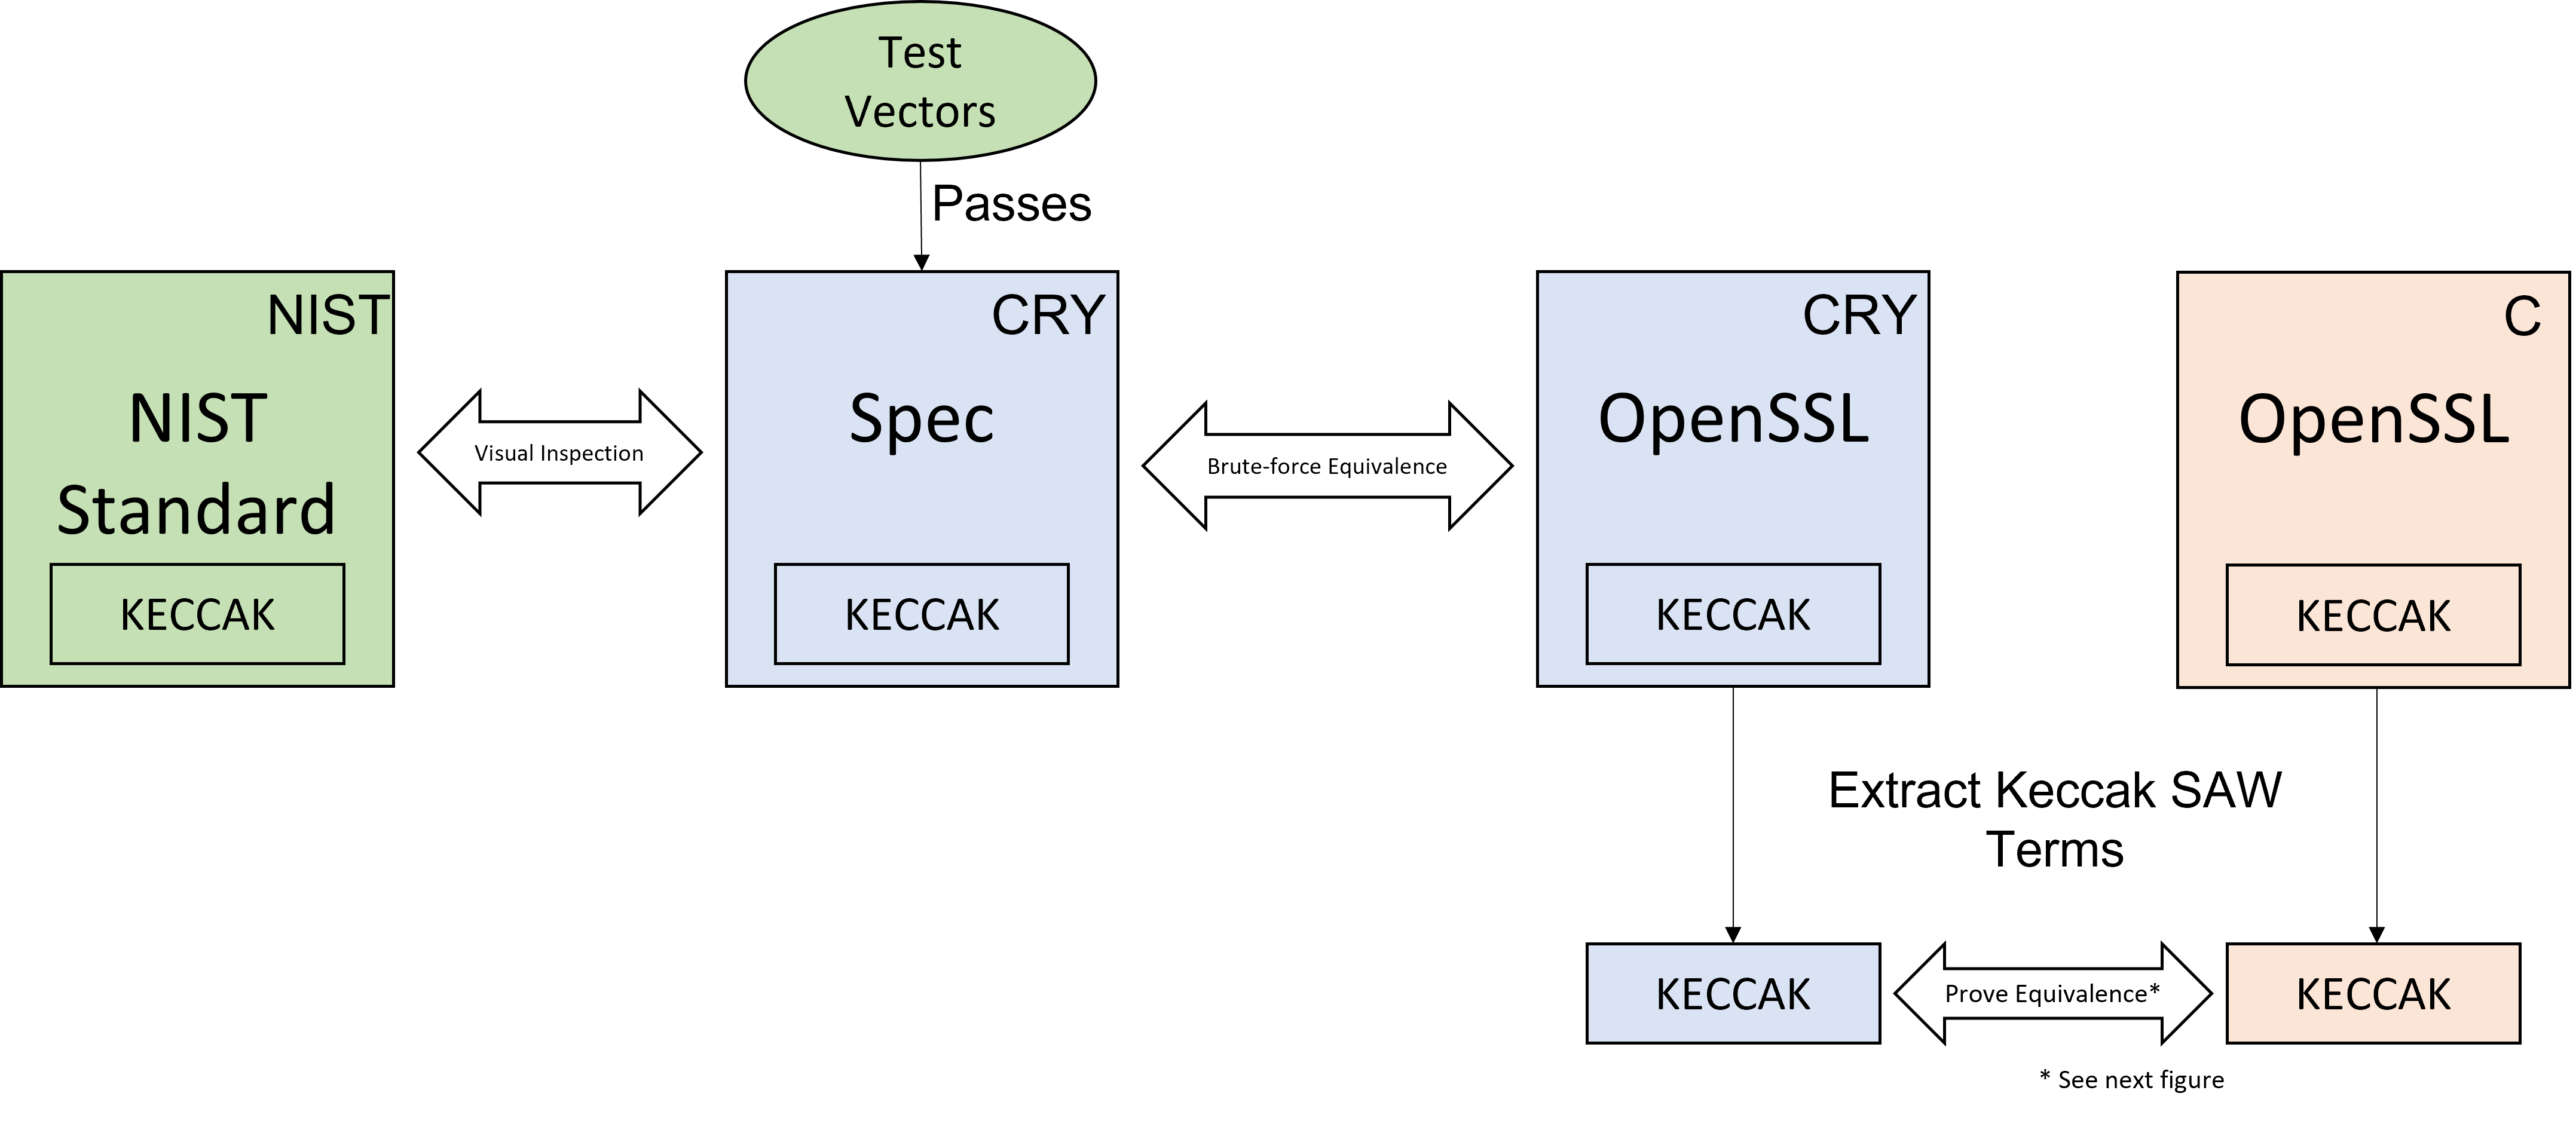
\includegraphics[width=\linewidth]{figs/proof.png}
  
  \caption{SHA3 Keccak Proof Structure}
  \label{fig:proofStructure}
  
\end{figure*}
\begin{figure*}[ht]
  \centering
  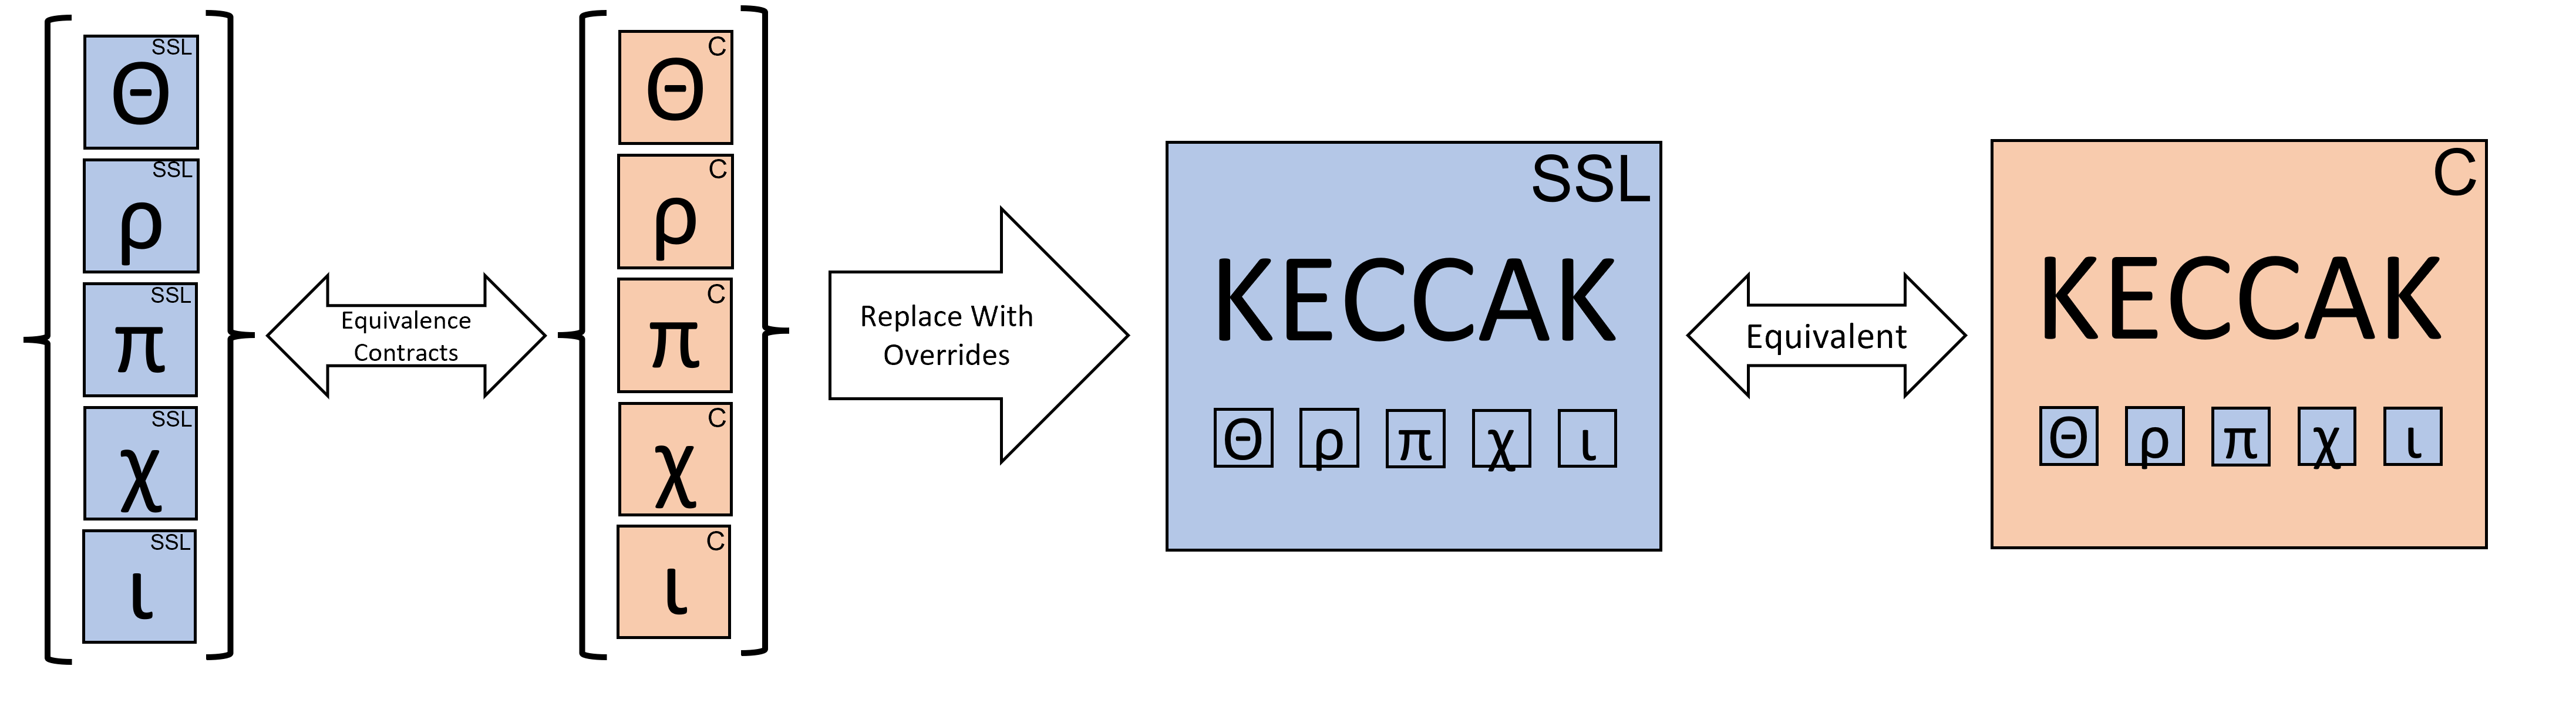
\includegraphics[width=\linewidth]{figs/proof2.png}
  
  \caption{Inner Function Contracts}
  \label{fig:proofStructure2}
  
\end{figure*}

\begin{compactitem}
  \item Process 1600 bits at a time: $5 * 5 * 64$
  \item State vector is $5*5*64*$
  \item Incoming message padded out to whole number of 1600 bit bit-strings
  \item Processed in order by \texttt{KECCAK}
  \item Keccak turns each block into a state vector (rearranges bit layout in memory)
  \item Keccak has 24 rounds for state vector. 
  \item There are 5 hash functions sequentially applied in each round to iteratively update the state vector
  \item After the last round, keccak turns the state vector back into the bit-string./\item The next unprocessed block is \emph{sponged} (e.g., absorbed) into the current bit-string from the latest keccak and the process is repeated 
  \item The max digest (hash) size is 512 bits in the standard
  \item The final bit-string from keccak after sponging and processing every block in the original message is truncated to the desired digest size 
\end{compactitem}

SAW Details
\begin{compactitem}
  \item Cryptol is a specification language specifically for defining crypto-primitives
  \item It has a compiler to turn Cryptol to SAW core terms
  \item It has an execution environment to run test vectors on specifications
  \item SAW is a tool to prove equivalence between SAW core terms
  \item It uses symbolic execution and must unroll every loop to a fixed length
  \item It can take as input C and Java code and compile those to core terms
  \item It can use overides to replace C and Java code in the term
\end{compactitem}

SAW provides a verification environment for compositional proofs of functional equivalence between two pieces of supported code (C, Java, or Cryptol).
SAW uses symbolic execution to create computational models of the code and creates problems of functional equivalence between those two models that can be pushed off to an SMT solver.  
The difficulty of these SMT problems is directly affected by the size and complexity of the computations that are being compared.
This can lead to drastic increases in proof times and sometimes even prevents completion as computations increase.  
SAW's solution to this is to create contracts (called overrides) of a functions input to output relationship which allows for a modular approach to writing the proof.
By breaking up computation into smaller pieces, and creating overrides for these pieces, SAW can often simplify an otherwise complex (and thus incompletable) proof to remain within the capacity of an SMT solver.

Cryptol is a domain-specific specification language, which has been used in the previously mentioned works by Galois' and by Decker et. al to write visually reviewable implementations of NIST standards.
It has strong ties to the SAW tool and, in fact, can be compiled directly down to the SAW Terms (computational models) which are used by SAW in proving functional equivalence.
Because of the interwoven nature of Cryptol with SAW, the Terms created from Cryptol are in most cases significantly simpler than any created through symbolic execution of C/Java code.

The published NIST standards provide no compileable implementation that can be used as a starting point for proving out the algorithm.
As a result, any proof of correctness with a NIST standard is limited in strength to how simple it is use visual review to connect code used in the proof to the NIST standard, coupled with a small sampling of test vectors.
As shown in \ref{proofStructure}, The proof flow starts with a specification of the SHA3 algorithm in Cryptol with the goal of being as similar visually to the NIST standard as possible.
This work discusses significant ways that Cryptol's functional nature can be leveraged to aid in this goal.
Along with simplifying the visual inspection process, this Cryptol specification also passes all test vectors provided by NIST.

The end goal of this proof is to show functional equivalence between this visually reviewable specifications Keccak function, and that of OpenSSL's C code.
Unfortunately, a direct proof between this specification, and OpenSSL's implementation proved unfeasible, because OpenSSL varies from the NIST standard in how it stores the bits of the intermediate state array in memory.
These minor modifications in memory storage put such a proof out of SAW's capabilities, because it relies on strict typing, and comparison of a Cryptol functions input/output to a C functions memory state.
In order to bridge that gap, a second Cryptol specification is included in the proof flow.
It matches in every way the first Cryptol code, except when it comes to how the state array is stored and accessed (at which point it follows OpenSSL's form).
Because of the efficient nature of Cryptol's compilation to SAW Terms, proving equivalence between these Cryptol implementations was possible at the top level of the SHA3 algorithm (which allows for the differences in state array storage to be fully abstracted out).
Due to the strict typing nature required for writing SAW proofs, the scope of this equivalence proof is limited to a given input message size.
The only computations that change in the SHA3 algorithm due to message size are in the padding and sponging of a block.
With this in mind, an exhaustive proof run over each input message byte count from 1 to the block size is sufficient to cover the differences in computation.
The artifact repository accompanying this work contains the receipts of this exhaustive proof. (REFERENCE TO PROOF!!!!)

INNER GREEK FUNCTIONS:

CONTRACTS CAN BE USED TO OVERRIDE AND REPLACE C WITH Cryptol

WITH THESE CONTRACTS SAW CAN COMPLETE A PROOF OF EQUIVALENCE BETWEEN TWO PIECES OF CODE.

This work relies on the correctness of several tools, including language compilers. 

\noindent \textbf{Trusted Code Base}:
\begin{itemize}
  \item LLVM bitcode compiler
  \item The Software Analysis Workbench (SAW) including the conversion from LLVM bitcode to SAWCore terms, the Cryptol compiler to SAWCore terms, and SAW's interface with SMT solvers.
  \item The z3, abc, and yices SMT solvers.
\end{itemize}

\section{Amended Cryptol}\label{sec:amended}
TODO:

Imperative spec, functional language, Cryptol's looping syntax can be cryptic.

Rational and descriptions of utility functions, examples of utility functions.

for-each == javascript map, while loop == javascript reduce.

Initially it appeared that visual inspection with Cryptol’s standard syntax was subpar.
Cryptol’s functional folds and list comprehensions do not align easily with the imperative 
and array-based NIST standard. BY leveraging Cryptol’s versatility, however, we produced a couple 
utility functions to visually mimic the sequential nature of the specification. 

The phrase “for all” is quite common in the NIST document, and it implies a looping structure. 
The following is the NIST definition of the pi function:
\begin{verbatim}
  1. For all triples (x,y,z) such that 
    0 <= x < 5, 0 <= y < 5, and 0 <= z < w,
    let A'[x, y, z] = A[(x + 3y) mod 5, x, z].
  2. Return A'.
\end{verbatim}
    
Using Cryptol's list comprehensions, we find the following syntax for the pi function:
\begin{verbatim}
  type COL = 5 
  type W = 64
  LIST4 = [0..COL-1]
  LIST63 = [0..W-1]
  type STATE_ARR = [COL][COL][W]
  pi : STATE_ARR -> STATE_ARR
  pi a = [[[a @x @((x + 3y) % COL) @z 
             | z <- LIST63] 
           | y <- LIST4] 
         | x <- LIST4]
\end{verbatim}

Cryptol declares list comprehension variables after they are used, and the order of the
nested loops is not as apparent. Using a helper function, ‘for’, we were able to provide
the following syntax:

\begin{verbatim}
  type COL = 5 
  type W = 64
  type STATE_ARR = [COL][COL][W]
  LIST4 = [0..COL-1]
  LIST63 = [0..W-1]
  pi : STATE_ARR -> STATE_ARR
  pi a = for LIST4 (\y ->
           for LIST4 (\x -> 
             for LIST4 (\z -> 
               a @x @((x + 3*y) % `COL) @z)))
\end{verbatim}

  The ‘for’ utility function follows the same intuition as the implementation in most 
  imperative languages. That is, it iterates over the list provided. It is similar to the 
  Array.prototype.map method in JavaScript in that it takes in a function and a list of 
  arguments and returns a list of results from calling the function on every element of the 
  input array. It is implemented as so:

\begin{verbatim}
  for : {n, a, b} [n]a -> (a -> b) -> [n]b
  for vals loop = [loop index | index <- vals]
\end{verbatim}

While simple to implement, it reorders and structures the arguments in a very elegant way.
In constrast with standard cryptol syntax, the list to iterate over and the iterating 
variable are visible before the loop body. List comprehensions are hidden away behind this 
function call and visual equivalence is clearer.

Another common phrasing is the “let...for...let”. This defines a state upon which a folding 
occurs, which is most comparable to a while loop. Here is the rc function as defined in the 
NIST spec:

\begin{verbatim}
  1. If t mod 255 = 0, return 1.
  2. Let R = 10000000.
  3. For i from 1 to t mod 255, let:
    a. R = 0 || R;
    b. R[0] = R[0] ^ R[8];
    c. R[4] = R[4] ^ R[8];
    d. R[5] = R[5] ^ R[8];
    e. R[6] = R[6] ^ R[8];
    f. R =Trunc8[R].
  4. Return R[0].
\end{verbatim}

Cryptol list comprehensions require a list to iterate over. Our ‘for’ utility function does 
as well. Knowing that the number of iterations is bounded by [1, 254], we can construct the 
following ungainly Cryptol definition:

\begin{verbatim}
  rc : [64] -> Bit
  rc t = if (t % 255) == 0 
    then True 
      else (rList !0).R @0 where
        rList = [{i = 1, R = 128:[8]}] # [{
          i = r @i + 1, 
          R = if i <= t % 255
            then (take`{8} ([
              (r@0)^(r@8),
              r@1,
              r@2,
              r@3, 
              (r@4)^(r@8),
              (r@5)^(r@8),
              (r@6)^(r@8),
              r@7,
              r@8])
                where r = [False] # state.R)
            else (rList @i).R}
          | i <- [0..254]]
\end{verbatim}

Not only is this computationally slower since it runs 255 loops every time rc is called,
it differs vastly from the NIST specificiation. Using a new ‘while’ utility function, we 
can declare an initial state, condition function, and body function that will recursively 
be called until the condition is met. Here is the rc function with the use of this utility 
function:

\begin{verbatim}
  rc : [64] -> Bit
  rc t = if (t % 255) == 0 
    then True 
    else (while {i = 1, R = 128:[8]} //STATE
      (\state -> state.i <= t % 255) //COND
      (\state -> {                   //LOOP
        i = state.i + 1, 
        R = (take`{8} ([
          (r@0)^(r@8),
          r@1,
          r@2,
          r@3,
          (r@4)^(r@8),
          (r@5)^(r@8),
          (r@6)^(r@8),
          r@7, 
          r@8]) 
            where r = [False] # state.R)})
      ).R @0
\end{verbatim}

The final state is returned by the ‘while’ function. This iterates only until the 
condition is met, avoids the clutter of indexing within a larger array of all previous 
states, and places the condition in a more obvious location before the loop body. Here 
is the definition of the ‘while’ utility function:

\begin{verbatim}
  while : {a} a -> (a -> Bit) -> (a -> a) -> a
  while state cond f = if (cond state)
    then (while (f state) cond f)	
    else state
\end{verbatim}

While the condition is not met by the current state, continue to iterate. Else, return the 
current state.

\section{Static Iota}\label{sec:iota}
NIST specification invokes the rc method seven times for each iota function call.
As the rc inputs are the same for each round, OpenSSL's optimized implementation of keccak stores 
the output values as a constant table. Initially, we matched out Cryptol execution of the NIST standard 
as closely as possible--including rc method calls in the iota function. We soon found that SAW was unable 
to map our implementation of keccak to OpenSSL's without the use of a constant table.
Our final Cryptol implementation uses the rc definition found in the NIST specification to generate a table 
that is easiy compared to OpenSSL. This allows SAW to generate a proof and permits visual inspection of equivalence.
\section{Visual Limitations}\label{sec:visual}
Talk about visual Limitations
\subsection{Iota}
Have to make small concession because we do prove that it computes all 24 values using rc, but it does it in one swoop still, rather than as needed.

Assert function is not useable in the Symbolic Execution Engine.
To fix this, we replace it with an if statement that checks the same expression and only runs code if it returns true.
\subsection{Array Storage}
OpenSSL switches the ordering of their x/y's for the array.
Because we're proving the small inner parts of the code, we have to match memory structures.

Whatever we decided for the bit reversal (still might try to get a cryptol->cryptol proof running).
Add conclusions and future work.


%%
%% The acknowledgments section is defined using the "acks" environment
%% (and NOT an unnumbered section). This ensures the proper
%% identification of the section in the article metadata, and the
%% consistent spelling of the heading.
\begin{acks}
To Robert, for the bagels and explaining CMYK and color spaces.
\end{acks}

%%
%% The next two lines define the bibliography style to be used, and
%% the bibliography file.
\bibliographystyle{ACM-Reference-Format}
\bibliography{paper.bib}

\end{document}
\endinput
%%
%% End of file `paper.tex'.
